
\chapter{Multivariate Models}
\label{chap:multivariate}

Despite the existing approaches in the literature, dealing with multivariate and spatio-temporal time series was always a challenging task for FTS methods, specially because of the complexity growth of the rules as the dimension increases. An important gap in the literature is the absence of multiple input and multiple output (MIMO) methods - the majority of FTS literature consists of basically univariate forecasting methods.  

A simple approach is to transform multivariate time series into monovariate time series by using Fuzzy Information Granules (FIG). Each FIG acts as a multivariate fuzzy set, or a composition of individual fuzzy sets from different variables, allowing to replace a vector (the values of one data point) by a scalar (the identification of the FIG with the highest membership of that data point).

This approach is employed on Fuzzy Information Granular Fuzzy Time Series ($\FIG$-FTS), a wrapper method that enables PWFTS to tackle multivariate time series. It begins by partitioning the Universe of Discourse of each individual variable. Then the crisp values of each variable are fuzzyfied and the corresponding fuzzy sets are combined to create one Fuzzy Information Granule, such that it can be used as a reference of all data points in that same region. This incremental approach creates the FIGs on demand, according to the training data, and its sensibility can be controlled using the method's hyperparameters. 

This chapter presents a short review of multivariate FTS methods and Fuzzy Information Granules in Section \ref{sec:fts_multivariate}. Section \ref{sec:mvfts} presents a conventional method for multivariate FTS (MVFTS), which does not employ FIGs. In Section \ref{sec:fig_fts} the Fuzzy Information Granule Fuzzy Time Series ($\FIG$-FTS) is proposed to enable PWFTS method be used for multivariate data and allowing the use of its interval and probabilistic forecasting features. In Section \ref{sec:multivariate_experiments} an exploratory study of the performance of $\FIG$-FTS when compared with previous FTS methods is presented and finally, in Section \ref{sec:multivariate_conclusion}, the results are discussed and the conclusions given. 


%%%%%%%%%%%%%%%%%%%%%%%%%%%%%%%%%%%%%%%%%%%%%%%%%%%%%%%%%%%%%
%%%%%%%%%%%%%%%%%%%%%%%%%%%%%%%%%%%%%%%%%%%%%%%%%%%%%%%%%%%%%
\section{Multivariate FTS Methods}
\label{sec:fts_multivariate}

Multivariate time series are sets of sequential vectors of the form $Y \in \mathbb{R}^n$ where $n = |\var|$ and $\var$ is the set of attributes of $Y$. Each vector $y(t) \in Y$ contains all attributes $\vari \in \var$ and there is a temporal dependence between these data points such that their temporal ordering -- given by the time index $t \in T$ -- must be respected. 

In the FTS literature it is common to employ clusterization methods to reduce multivariate data in monovariate ones, as can be seen in \cite{Li2008b}, \cite{Chen2010}, \cite{Sun2015} which employ Fuzzy C-Means (FCM) clustering algorithm to create multivariate FLRG's.

\cite{Chen2011} introduced the concept of \textit{Fuzzy Variation Groups} - FVG for bivariate FTS, where each FVG groups the FLRG's of each variable by their co-occurrence. \cite{Askari2015} proposes the \textit{High-Order Multi-Variable FTS} - HMV-FTS algorithm based on FCM clustering to generate the multi-variable FLRG's. \cite{Jilani2008} proposed the \textit{Multivariate Stochastic FTS} - MSFTS based on the exponential smoothing between the diverse variables.

\subsection{Fuzzy Information Granules}

The concept of Fuzzy Information Granules (FIG) was first proposed in \cite{Zadeh1996} as a way to define entities that represent subsets (or granules) of a wider domain. There are some works in the FTS literature where this concept is mixed with the partition of the Universe of Discourse, as discussed in \cite{Lu2014, Chen2015}, but there are several ways to define FIG in the literature. 

For univariate time series it is common to define a FIG as representative set of sub-samples of the data, so each FIG is a common temporal pattern as in \cite{Yang2017b}. The construction of this kind of FIG usually employs the clustering of sub-sequences, as in \cite{Magalhaes2008}. In \cite{Wang2014a, Wang2015} we can find a univariate fuzzy time series approach whose FIGs are a combination of unequal partitioning of the UoD and prototype sub-sequences. 

For multivariate time series FIGs are usually represented as hyper-boxes or multidimensional clusters in the feature space, as in \cite{Reyes-Galaviz2016, Singh2018}.  In \cite{Singh2018},  a multivariate fuzzy time series method is presented, which uses a bio-inspired optimization method to create FIGs by iteratively adjusting the interval lengths of each variable.

Other non-FTS granular approaches can also be found in the literature, as the Granular Functional Forecasting (GFM), proposed in \cite{Magalhaes2008}, a univariate forecasting method based on Takagi-Sugeno fuzzy system where FIGs are created using clustering methods. In \cite{Leite2011}, the authors propose the fuzzy set  based  granular  evolving modeling (FBeM) approach for time series prediction, later extended in \cite{Soares2018} for spatio-temporal data.

There are some notable drawbacks in the previous methods, namely: a) the absence of multivariate forecast (MIMO); b) the use of optimization methods to create the FIGs, which makes the learning process computationally expensive; c)~the absence of multivariate FTS methods that could provide both weighted and high order characteristics. To fix these drawbacks this work proposes the $\mathcal{FIG}$-FTS method, a weighted and high-order FTS method that will be discussed in the next sections. 

%%%%%%%%%%%%%%%%%%%%%%%%%%%%%%%%%%%%%%%%%%%%%%%%%%%%%%%%%
%%%%%%%%%%%%%%%%%%%%%%%%%%%%%%%%%%%%%%%%%%%%%%%%%%%%%%%%%
\section{The Conventional Multivariate Fuzzy Time Series method}
\label{sec:mvfts}

Just as it was done in Chapter \ref{chap:review_fts}, this section proposes a consensus model for rule based multivariate FTS that extends the model of \cite{chen1996forecasting} to the multivariate case. The Conventional Multivariate Fuzzy Time Series (MVFTS) method was designed to allow several models to be trained individually with subsets of a greater dataset and later to be merged into a single model, feature that enhances the performance of model creation by enabling its distribution.

For each chosen variable $\vari \in \var$ on $Y$, MVFTS also incorporates several features present in the literature, represented by the hyperparameters in Table~\ref{tab:mvfts_hyperparameters}, giving versatility and flexibility to the model. The method is composed of two procedures: the training procedure and the forecasting procedure.

\begin{table}[]
    \centering
    \begin{tabular}{|c|m{2cm}|c|m{.5\textwidth}|} \hline
        \textbf{Alias} & \textbf{Parameter} & \textbf{Type} & \textbf{Description}  \\ \hline
         $k_i$ & Number of partitions & $\mathbb{N}^+$ & The number of fuzzy sets that will be created in the linguistic variable $\mlvar$  \\ \hline
         $\mu$ & Membership function & $\mu: U \rightarrow [0,1] $ & A function that measure the membership of a value $y \in U$ to a fuzzy set  \\\hline
         $\alpha$ & $\alpha$-cut & $[0,1]$ & The minimal membership grade to take account on fuzzyfication process \\ \hline
    \end{tabular}
    \caption{WMVFTS hyperparameters for each variable $\vari \in \var$}
    \label{tab:mvfts_hyperparameters}
\end{table}

The MVFTS is a first order point forecaster of type Multiple Input/Single Output (MISO), then for the set of variables $\var$ one of them is chosen as the target (or endogenous) variable and the others are referred as the explanatory (or exogenous) variables. From now on, the target variable will be distinguished from the others by an asterisk, as $*\var$.

The training procedure, explained in subsection \ref{sec:mvfts_training_procedure} and illustrated in Figure~\ref{fig:mvfts_training_procedure}, is a three stage process responsible to create a multivariate weighted FTS model $\model$. The final MVFTS model  $\model$ consists of a set of variables $\var$, a fuzzy linguistic variable $\mlvar$ for each $\vari \in \var$ and a set of weighted fuzzy rules over the linguistic variables $\mlvar$. The inputs of the training procedure are the crisp time series training data $Y$ and the set of hyperparameters for each $\vari \in \var$.

The forecasting procedure, explained in subsection \ref{sec:mvfts_forecasting_procedure} and illustrated in Figure~\ref{fig:mvfts_forecasting_procedure}, aims to produce a point estimate $\estimate$ for the target variable $*\var$, given an input sample $Y$, using the linguistic variables $\mlvar$ and the induced fuzzy rules on model $\model$.

%%%%%%%%%%%%%%%%%%%%%%%%%%%%%%%%%%%%%%%%%%%%%%%%%%%%%%%%%
%%%%%%%%%%%%%%%%%%%%%%%%%%%%%%%%%%%%%%%%%%%%%%%%%%%%%%%%%
\subsection{Training Procedure}
\label{sec:mvfts_training_procedure}

\begin{figure}
\centering
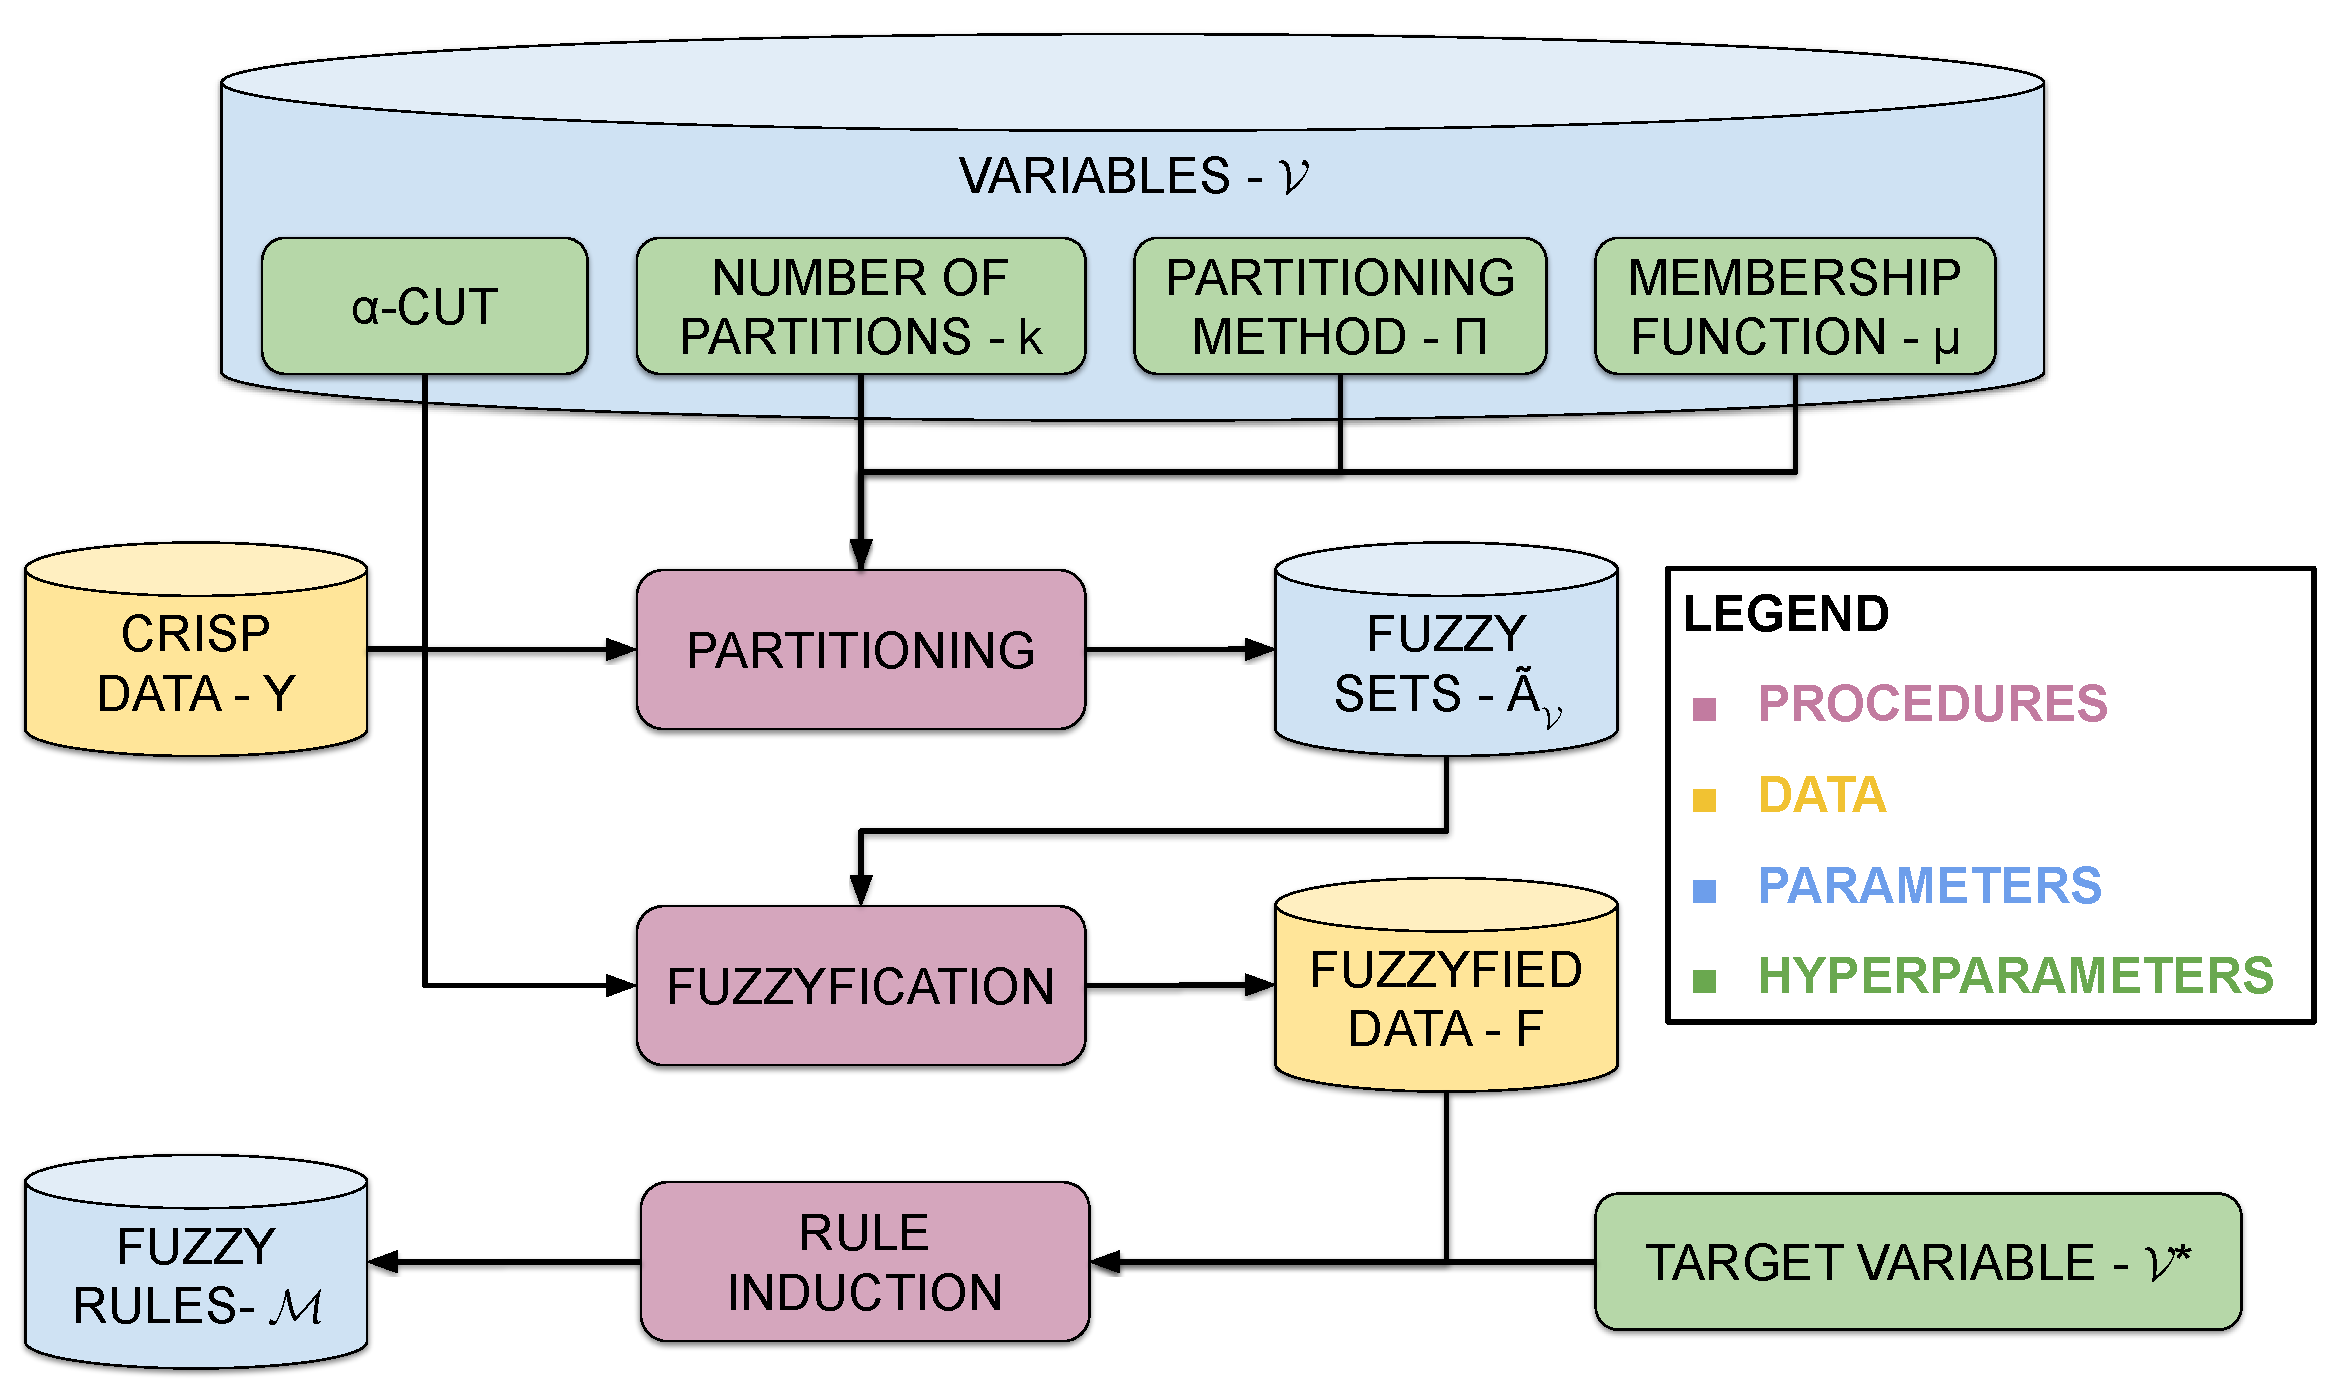
\includegraphics[width=\textwidth]{figures/mvfts_training_procedure.pdf}
\caption{MVFTS training procedure} \label{fig:mvfts_training_procedure}
\end{figure}

\begin{enumerate}
\item[Stage 1] \textit{Partitioning}:
\begin{enumerate}
\item \textit{Defining $U_{\vari}$}: The Universe of Discourse $U_{\vari}$ defines the sample space, i.e., the known bounds of the variable $\vari$, such that $U_{\vari} = [\min(Y^{\vari})-D_1, \max(Y^{\vari})+D_2]$, where $D_1 = \min(Y^{\vari})\times 0.2$ and $D_2 = \max(Y^{\vari})\times 0.2$ are used to extrapolate the known bounds as a security margin, $\forall \vari \in \var$.

\item \textit{$U_{\vari}$ Partitioning}: Split $U_{\vari}$ in $k_i$ intervals $U_j$ with midpoints $c_j$, for $j=0..k_i$, where all the intervals have the same length;

\item \textit{Define the linguistic variable $\mlvar$}: For each interval $U_j \in U_{\vari}$  create an overlapping fuzzy set $\mfset$, with the membership function $\mu_{\mfset}$. The midpoint of the fuzzy set $\mfset$ will be $c_j$, the lower bound $l_j = c_{j-1}$ and the upper bound $u_j = c_{j+1}$ $\forall$ $j >0$ and $j < k_i$, and $l_0 = \min U_{\vari}$, $l_k = \max U_{\vari}$. Each fuzzy set $\mfset$ is a linguistic term of the linguistic variable $\mlvar$;
\end{enumerate}

\item[Stage 2] \textit{Fuzzyfication}: 

Transform the original numeric time series $Y$ into a fuzzy time series $F$, where each data point $f(t) \in F$ is an $n \times k$ array with the fuzzyfied values of $y(t) \in Y$ with respect to the linguistic terms $\mfset \in \mlvar$, where the fuzzy membership is greater than the predefined $\alpha$-cut, i.e., $f(t) = \{\mfset\; |\; \mu_{\mfset}(y(t)^{\vari}) \geq \alpha_i\;\forall \mfset \in \mlvar\}$;

\item[Stage 3] \textit{Rule Induction}: 
\begin{enumerate}
\item \textit{Generate the temporal patterns}: The fuzzy temporal patterns associate the fuzzyfied values $\var$ to a set of possible values of the target variable $*\var$, such that $\var \rightarrow *\var$, whith the format $A_j^{\var_0},...,A_j^{\var_n} \rightarrow A_j^{*\var}$, where the precedent, or left hand side (LHS), is $f(t - 1) = \mfset, \forall \vari \in \var$, and the consequent, or right hand side (RHS), is $f(t+1) = \tfset$, $\tfset \in \tlvar$.

\item \textit{Generate the rule base}: Select all temporal patterns with the same precedent and group their consequent sets  creating a rule with the format $\var \rightarrow w_k \cdot A_k^{*\var}, w_j \cdot A_j^{*\var},...$, where the LHS is $f(t - 1) = \mfset, \forall \vari \in \var$ and the RHS is $f(t+1) \in \{A_k^{*\var},A_j^{*\var},... \}$. Each rule can be understood as the weighted set of possibilities which may happen on time $t+1$ (the consequent) when a certain precedent $A_{i0},...,A_{i\Omega}$ is identified on previous lag (the precedent).
\end{enumerate}
\end{enumerate}


%%%%%%%%%%%%%%%%%%%%%%%%%%%%%%%%%%%%%%%%%%%%%%%%%%%%%%%%%
%%%%%%%%%%%%%%%%%%%%%%%%%%%%%%%%%%%%%%%%%%%%%%%%%%%%%%%%%
\subsection{Forecasting Procedure} 
\label{sec:mvfts_forecasting_procedure}

\begin{figure}
\centering
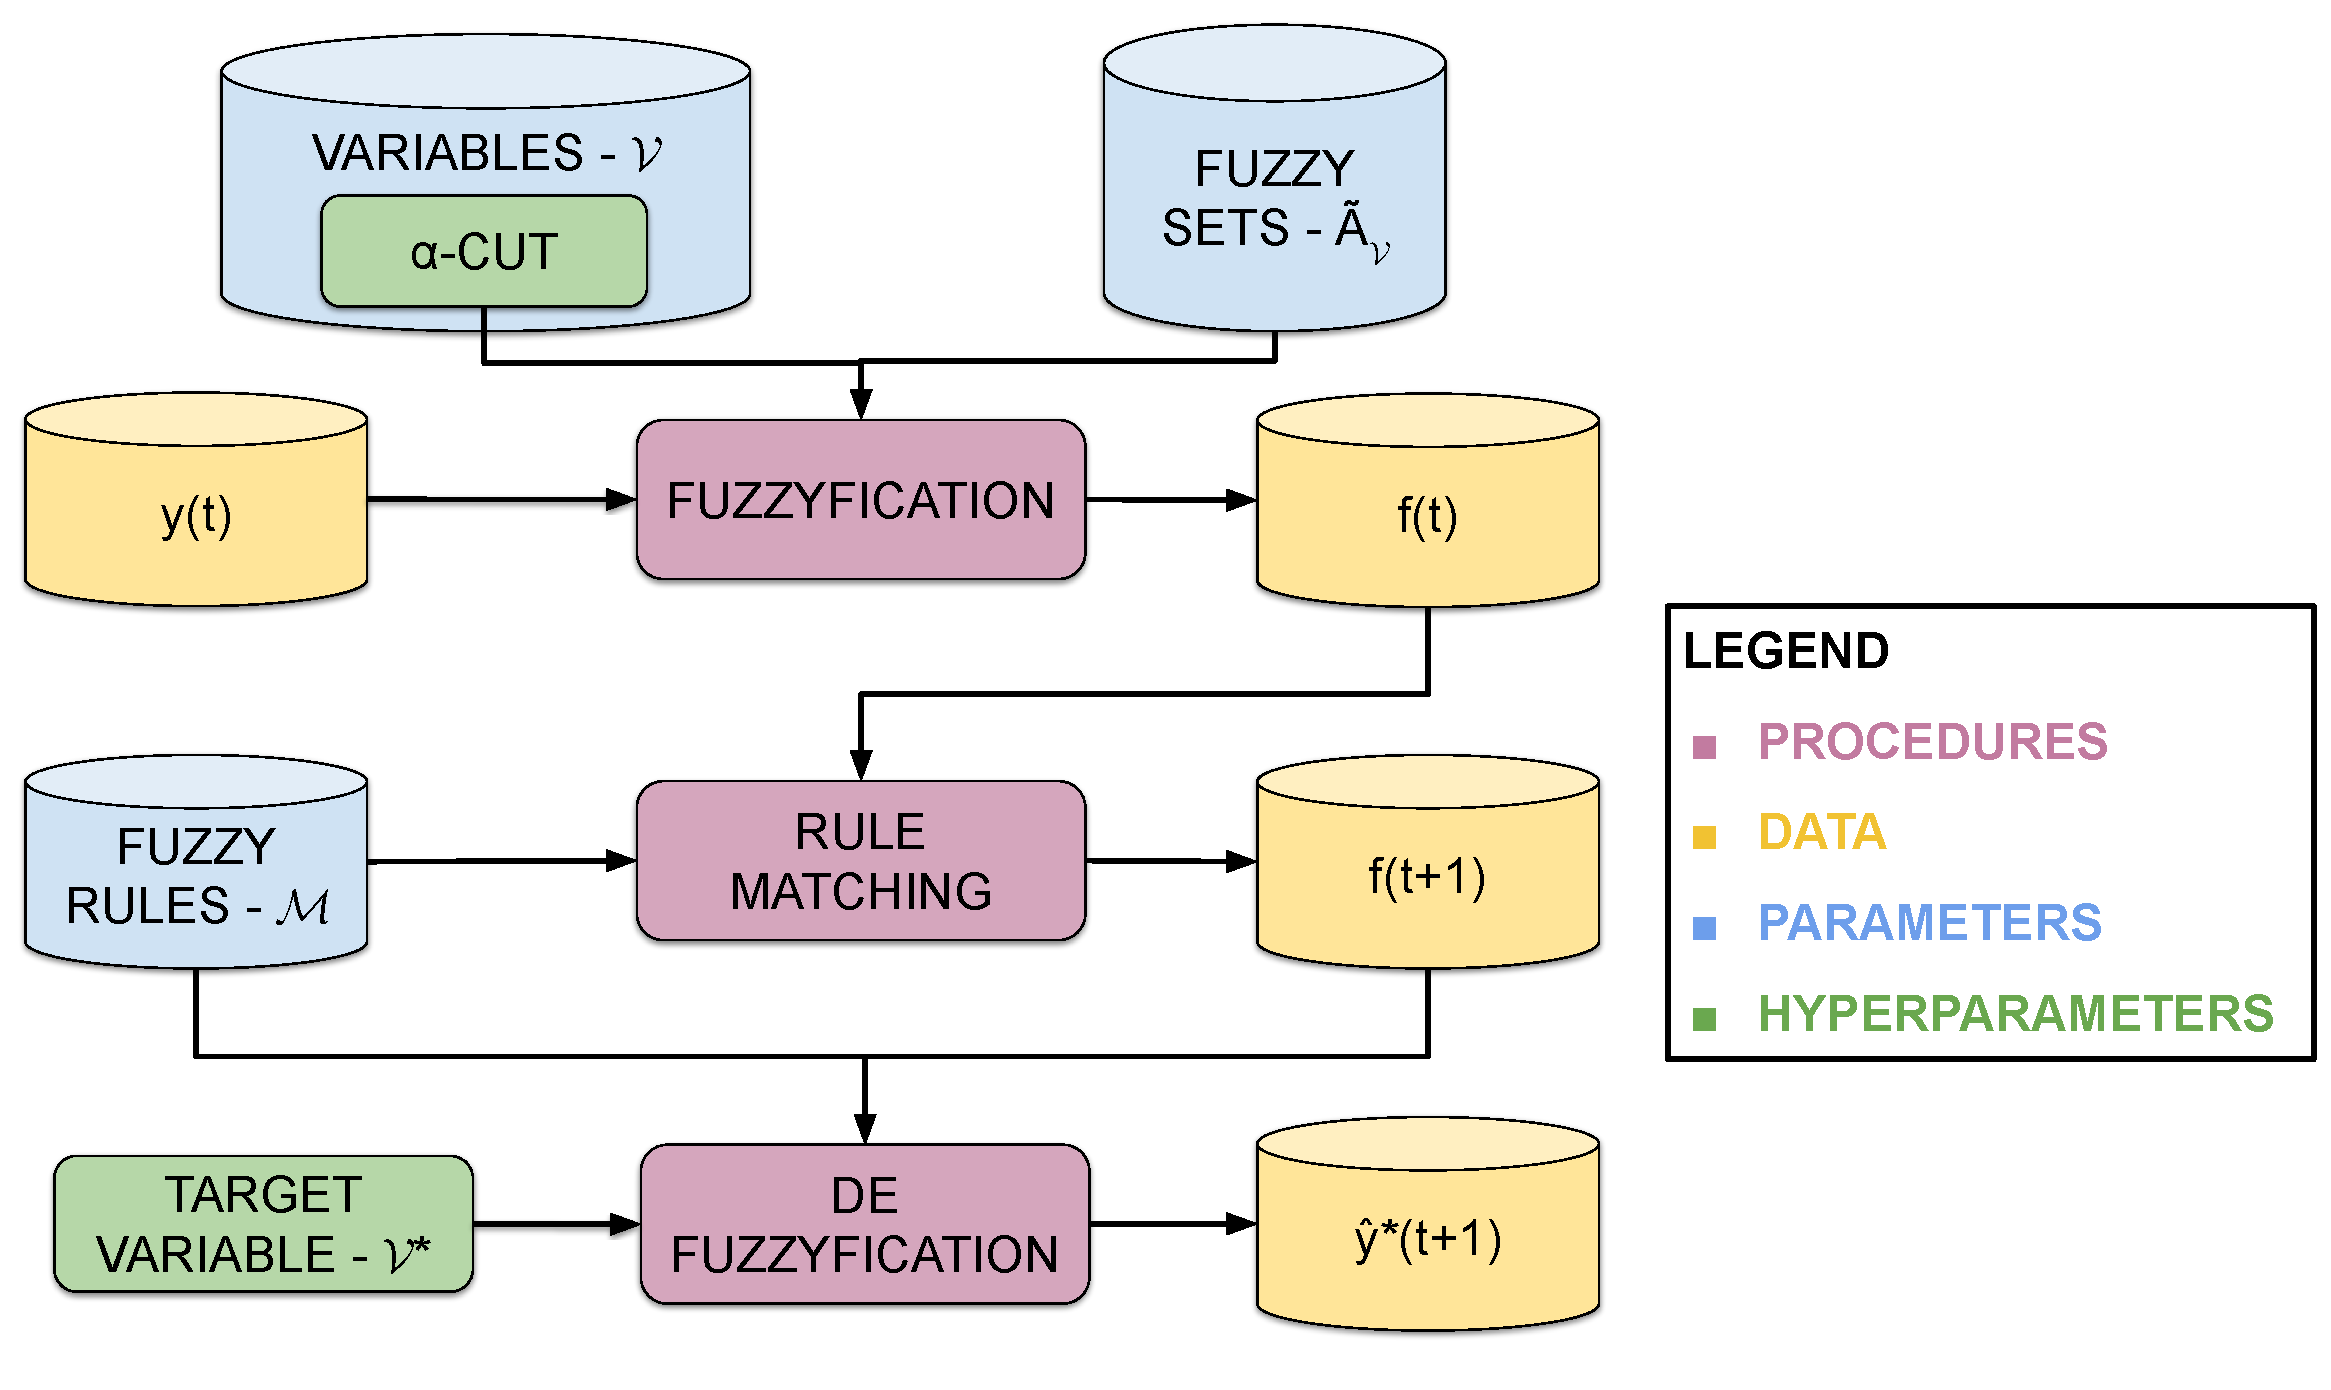
\includegraphics[width=\textwidth]{figures/mvfts_forecasting_procedure.pdf}
\caption{MVFTS forecasting procedure} \label{fig:mvfts_forecasting_procedure}
\end{figure}

\begin{enumerate}
\item [Step 1] \textit{Fuzzyfication}: Compute the membership grade $\mu_{ji}$ for $y(t-1) \in Y$ such that $\mu_{ji} = \mu_{\mfset}(y(t-1))$, for each $\mfset \in \mlvar$, for each $\vari \in \var$ ;
\item [Step 2] \textit{Rule matching}: Select the $K$ rules where all fuzzy sets $\mfset$ on the LHS, for each $\vari \in \var$, have $\mu_{ji} > \alpha_i$; The rule fuzzy membership grade is shown below, using the minimum function as T-norm.
\begin{equation}
    \mu_q = \bigcap_{j \in \mlvar\; ; \; i \in \var} \mu_{ji}
\end{equation}
\item [Step 3] \textit{Rule mean points}: For each selected rule $q$, compute the mean point $mp_q$ of the target variable $*\var$ as below, where $c_j$ is the $c$ parameter of the $\mu$ function from fuzzy set $\tfset$:
\begin{equation}
mp_q = \sum_{j \in *\mlvar} c_j
\end{equation}
\item [Step 4] \textit{Defuzzyfication}: Compute the forecast as the weighted sum of the rule mid-points $mp_q$ by their membership grades $\mu_q$ for each selected rule $j$:
\begin{equation}
\estimate = \frac{\sum_{q \in K} \mu_q \cdot mp_q}{\sum_{q \in K} \mu_q}
\end{equation}
\end{enumerate}

%%%%%%%%%%%%%%%%%%%%%%%%%%%%%%%%%%%%%%%%%%%%%%%%%%%%%%%%%
%%%%%%%%%%%%%%%%%%%%%%%%%%%%%%%%%%%%%%%%%%%%%%%%%%%%%%%%%
\subsection{Interval forecasting for MVFTS}
\label{sec:mvfts_interval}

The MVFTS model can be used for interval forecasting following the same approach of $\ifts$ method. For this it is needed to change the Steps 3 and 4 of the forecasting procedure presented in Section \ref{sec:mvfts_forecasting_procedure}, as presented below:

\begin{enumerate}
\item [Step 3] \textit{Rule intervals}: For each selected rule $q$, compute the interval $\intvl^q$ of the target variable $*\var$ as below, where $\underline{\tfset}$ and $\overline{\tfset}$ are respectively the lower and upper bounds of the target fuzzy sets  $\tfset$:
\begin{align}
    \intvl^q & =  [\underline{\intvl^q_{min}}, \overline{\intvl^q_{max}}] \\
    \underline{\intvl^q_{min}} &= \min(\underline{\tfset} \in *\mlvar) \\
    \overline{\intvl^q_{max}} &= \max(\overline{\tfset} \in *\mlvar) \\
\end{align}

\item [Step 4] \textit{Defuzzyfication}: Compute the prediction interval as the extrema of the rule intervals $\intvl_q$ by their membership grades $\mu_q$ for each selected rule $j$:
\begin{equation}
\mathbb{I}(t+1) = \frac{\sum_{j \in *\mlvar} \mu_q \mathbb{I}^q}{\sum_{q \in \var} \mu_q} = \frac{\sum_{q \in \var} [\mu_q\underline{\intvl^q_{min}} , \mu_q\overline{\mathbb{I}^q_{max}}] }{\sum_{q \in \var} \mu_q}
\label{eqn:mvifts}
\end{equation}
\end{enumerate}

%%%%%%%%%%%%%%%%%%%%%%%%%%%%%%%%%%%%%%%%%%%%%%%%%%%%%%%%%
%%%%%%%%%%%%%%%%%%%%%%%%%%%%%%%%%%%%%%%%%%%%%%%%%%%%%%%%%
\subsection{Weighted Multivariate FTS - WMVFTS}
\label{sec:wmvfts}

A simple extension of MVFTS to embody weights in its rules can be achieved by changing Stage 3.b of the training procedure presented in Section \ref{sec:mvfts_training_procedure}, where the new step is:

\begin{enumerate}
    \item[Stage 3.b)] \textit{Generate the rule base}: Select all temporal patterns with the same precedent and group their consequent sets  creating a rule with the format $\var \rightarrow w_k \cdot A_k^{*\var}, w_j \cdot A_j^{*\var},...$, where the LHS is $f(t - 1) = \mfset, \forall \vari \in \var$ and the RHS is $f(t+1) \in \{A_k^{*\var},A_j^{*\var},... \}$ and the weights $w_j, w_k, ...$ are the normalized frequencies of each temporal pattern such that:
\begin{equation}
w_i = \frac{\#\tfset}{\#RHS} \quad \forall \tfset \in RHS    
\end{equation}
where $\#A_i$ is the number of occurrences of $A_i$ on temporal patterns with the same precedent $LHS$ and $\#RHS$ is the total number of temporal patterns with the same precedent $LHS$.
\end{enumerate}

It is also need to change the Step 3 of the forecasting procedure presented in Section \ref{sec:mvfts_forecasting_procedure}, as presented below:

\begin{enumerate}
    \item [Step 3] \textit{Rule mean points}: For each selected rule $q$, compute the mean point $mp_q$ of the target variable $*\var$ as below, where $c_j$ is the $c$ parameter of the $\mu$ function from fuzzy set $\tfset$:
\begin{equation}
mp_q = \sum_{j \in *\mlvar} w_j \cdot c_j
\end{equation}
\end{enumerate}

For the interval forecasting method proposed in Section \ref{sec:mvfts_interval}, a new approach is adopted to create the fuzzy rule intervals, as presented below:

\begin{align}
    \intvl^q & =  [\underline{\intvl^q_{min}}, \overline{\intvl^q_{max}}] \\
    \underline{\intvl^q_{min}} &= \sum_{j \in *\mlvar} w_j \cdot \underline{\tfset} \\
    \overline{\intvl^q_{max}} &= \sum_{j \in *\mlvar} w_j \cdot \overline{\tfset} 
\end{align}

MVFTS and WMVFTS methods take separated partitionings for each variable and its rules contains references for the different variables.  In next section a simple approach is proposed for transforming multivariate time series in monovariate ones, allowing the use of monovariate FTS methods to tackle multivariate time series.

%%%%%%%%%%%%%%%%%%%%%%%%%%%%%%%%%%%%%%%%%%%%%%%%%%%%%%%%%%%%%
%%%%%%%%%%%%%%%%%%%%%%%%%%%%%%%%%%%%%%%%%%%%%%%%%%%%%%%%%%%%%
\section{Fuzzy Information Granule Fuzzy Time Series  $\FIG$-FTS}
\label{sec:fig_fts}
\index{Fuzzy Information Granules}\index{FIG-FTS}

The Fuzzy Information Granule Fuzzy Time Series ($\FIG$-FTS) is a wrapper model which enables a monovariate model (PWFTS) to tackle multivariate time series. In addiction to extending PWFTS features for multivariate data, the $\mathcal{FIG}$-FTS also appends the multivariate forecasting capability, acting as a Multiple Input/Multiple Output (MIMO) method, where all variables are both targets and explanatory variables. 

The aim of $\FIG$-FTS is to replace the Partitioning and Fuzzyfication stages of the PWFTS training procedure detailed in Section \ref{sec:pwfts_training}, the Fuzzyfication step of the forecasting procedure detailed in Section \ref{sec:pwfts_forecasting} and appends the multivariate forecasting to the extensions presented in Section \ref{sec:pwfts_extensions}.

Given an $n$-variate time series $Y=(y_1(t), \ldots,y_n(t)),  t=0\ldots,T$, corresponding variables $\var_i$ are defined for each $y_i(t)$. The resulting fuzzy time series $F$ is then composed by data points $f(t) \in F$ that represent a sequence of fuzzy information granules $\figi$. Each granule contains a set of fuzzy linguistic variables $\mlvar$ related to each variable $\var_i$.

The training procedure, described in Section \ref{sec:fig_training_procedure} and illustrated in Figure \ref{fig:figfts_training_procedure}, performs the multivariate partitioning, fuzzyfication and then feeds PWFTS with the fuzzyfied data, whose is responsible for rule induction. The final $\FIG$-FTS model $\model$ consists of a set of variables $\var$, a fuzzy linguistic variable $\mlvar$ for each $\vari \in \var$, a fuzzy information granule set $\FIG$ and a set of probabilistic weighted high order fuzzy rules over the information granules $\figi \in \fig$. The training procedure employ the hyperparameters listed in Table~\ref{tab:fig_hyperparameters}

In the training method the partitioning of each variable is independent from the others. Each variable has its own linguistic variable $\mlvar$. For this it is necessary to inform, for each chosen variable $\vari \in \var$ on $Y$, the hyperparameters $k_i, \mu$ and $\alpha$. The order of the model is controlled by the parameter $\Omega$ and the lag indexes are controlled by the parameter $L$. 

\begin{table}[]
    \centering
    \begin{tabular}{|c|m{2cm}|c|m{.5\textwidth}|} \hline
        \textbf{Alias} & \textbf{Parameter} & \textbf{Type} & \textbf{Description}  \\ \hline
         $k_i$ & Number of partitions & $\mathbb{N}^+$ & The number of fuzzy sets that will be created in the linguistic variable $\mlvar$  \\ \hline
         $\mu$ & Membership function & $\mu: U \rightarrow [0,1] $ & A function that measure the membership of a value $y \in U$ to a fuzzy set  \\\hline
         $\alpha$ & $\alpha$-cut & $[0,1]$ & The minimal membership grade to take account on fuzzyfication process \\ \hline
         $\Omega$ & Order & $\mathbb{N}^+$ & The number of past lags used in the precedent of each fuzzy rule \\\hline
         $L$ & Lags & & A vector of the past lag indexes, with length $\Omega$ and $1 \leq L[i] < L[i+1]$ for  $t=0..\Omega$ \\ \hline
         $\kappa$ & k-nearest neighbors & $\mathbb{N}^+$ & The number of nearest neighbors that the spatial index search on $\FIG$ during the fuzzyfication process \\ \hline
    \end{tabular}
    \caption{$\mathcal{FIG}$-FTS hyperparameters}
    \label{tab:fig_hyperparameters}
\end{table}

The global linguistic variable $\FIG$ is the union of all Fuzzy Information Granules $\figi$, which in turn are the combination of one fuzzy set for each variable, such that $\figi = \{ \mfset \}, \forall \vari \in \var$ and its membership function is given by $\mu_{\figi} = \bigcap \mu_{\mfset}$, where $\bigcap$ is the minimum T-norm. The $\FIG$ set is indexed by the midpoints of its internal fuzzy sets, enabling optimized spatial search using KD-trees.  
With the linguistic variable $\FIG$ the fuzzyfication process transforms each multivariate data point $y(t) \in Y$ into a  $\figi \in \FIG$, such that $f(t) = \figi$.

The forecasting procedure, explained in subsection \ref{sec:fig_forecasting_procedure} and illustrated in Figure \ref{fig:figfts_forecasting_procedure}, aims to produce a point estimate $\estimate$ for each variable $\var$, given an input sample $Y$, using the linguistic variable $\FIG$ and the induced fuzzy rules on model $\model$.

The rule matching procedure can become computationally expensive as the size of the rule base $\model$ grows. Because of this it is advisable that implementations of this model use spatial trees \citep{Muja2014} to index the rules with the midpoints of each fuzzy set on their $LHS$, optimizing the search for applicable rules during the forecasting step. This work used the KD-tree implementation of the Scipy Spatial package\footnote{\url{https://docs.scipy.org/doc/scipy/reference/spatial.html}. Access in 2019-04-29.}.

The global parameter $\kappa$ is related with the spatial index search on $\FIG$, and indicates how many $\figi \in \FIG$ are returned for a given crisp multivariate data point. This parameter has influence on the sensibility and the diversity of the rules considered during the forecasting procedure, such that as $\kappa$ increases more rules will be accounted on. If $\kappa = 1$, just the closest rule (the rule with the highest membership degree) will be used. 

%%%%%%%%%%%%%%%%%%%%%%%%%%%%%%%%%%%%%%%%%%%%%%%%%%%%%%%%%
%%%%%%%%%%%%%%%%%%%%%%%%%%%%%%%%%%%%%%%%%%%%%%%%%%%%%%%%%
\subsection{Training Procedure}
\label{sec:fig_training_procedure}

\begin{figure}
\centering
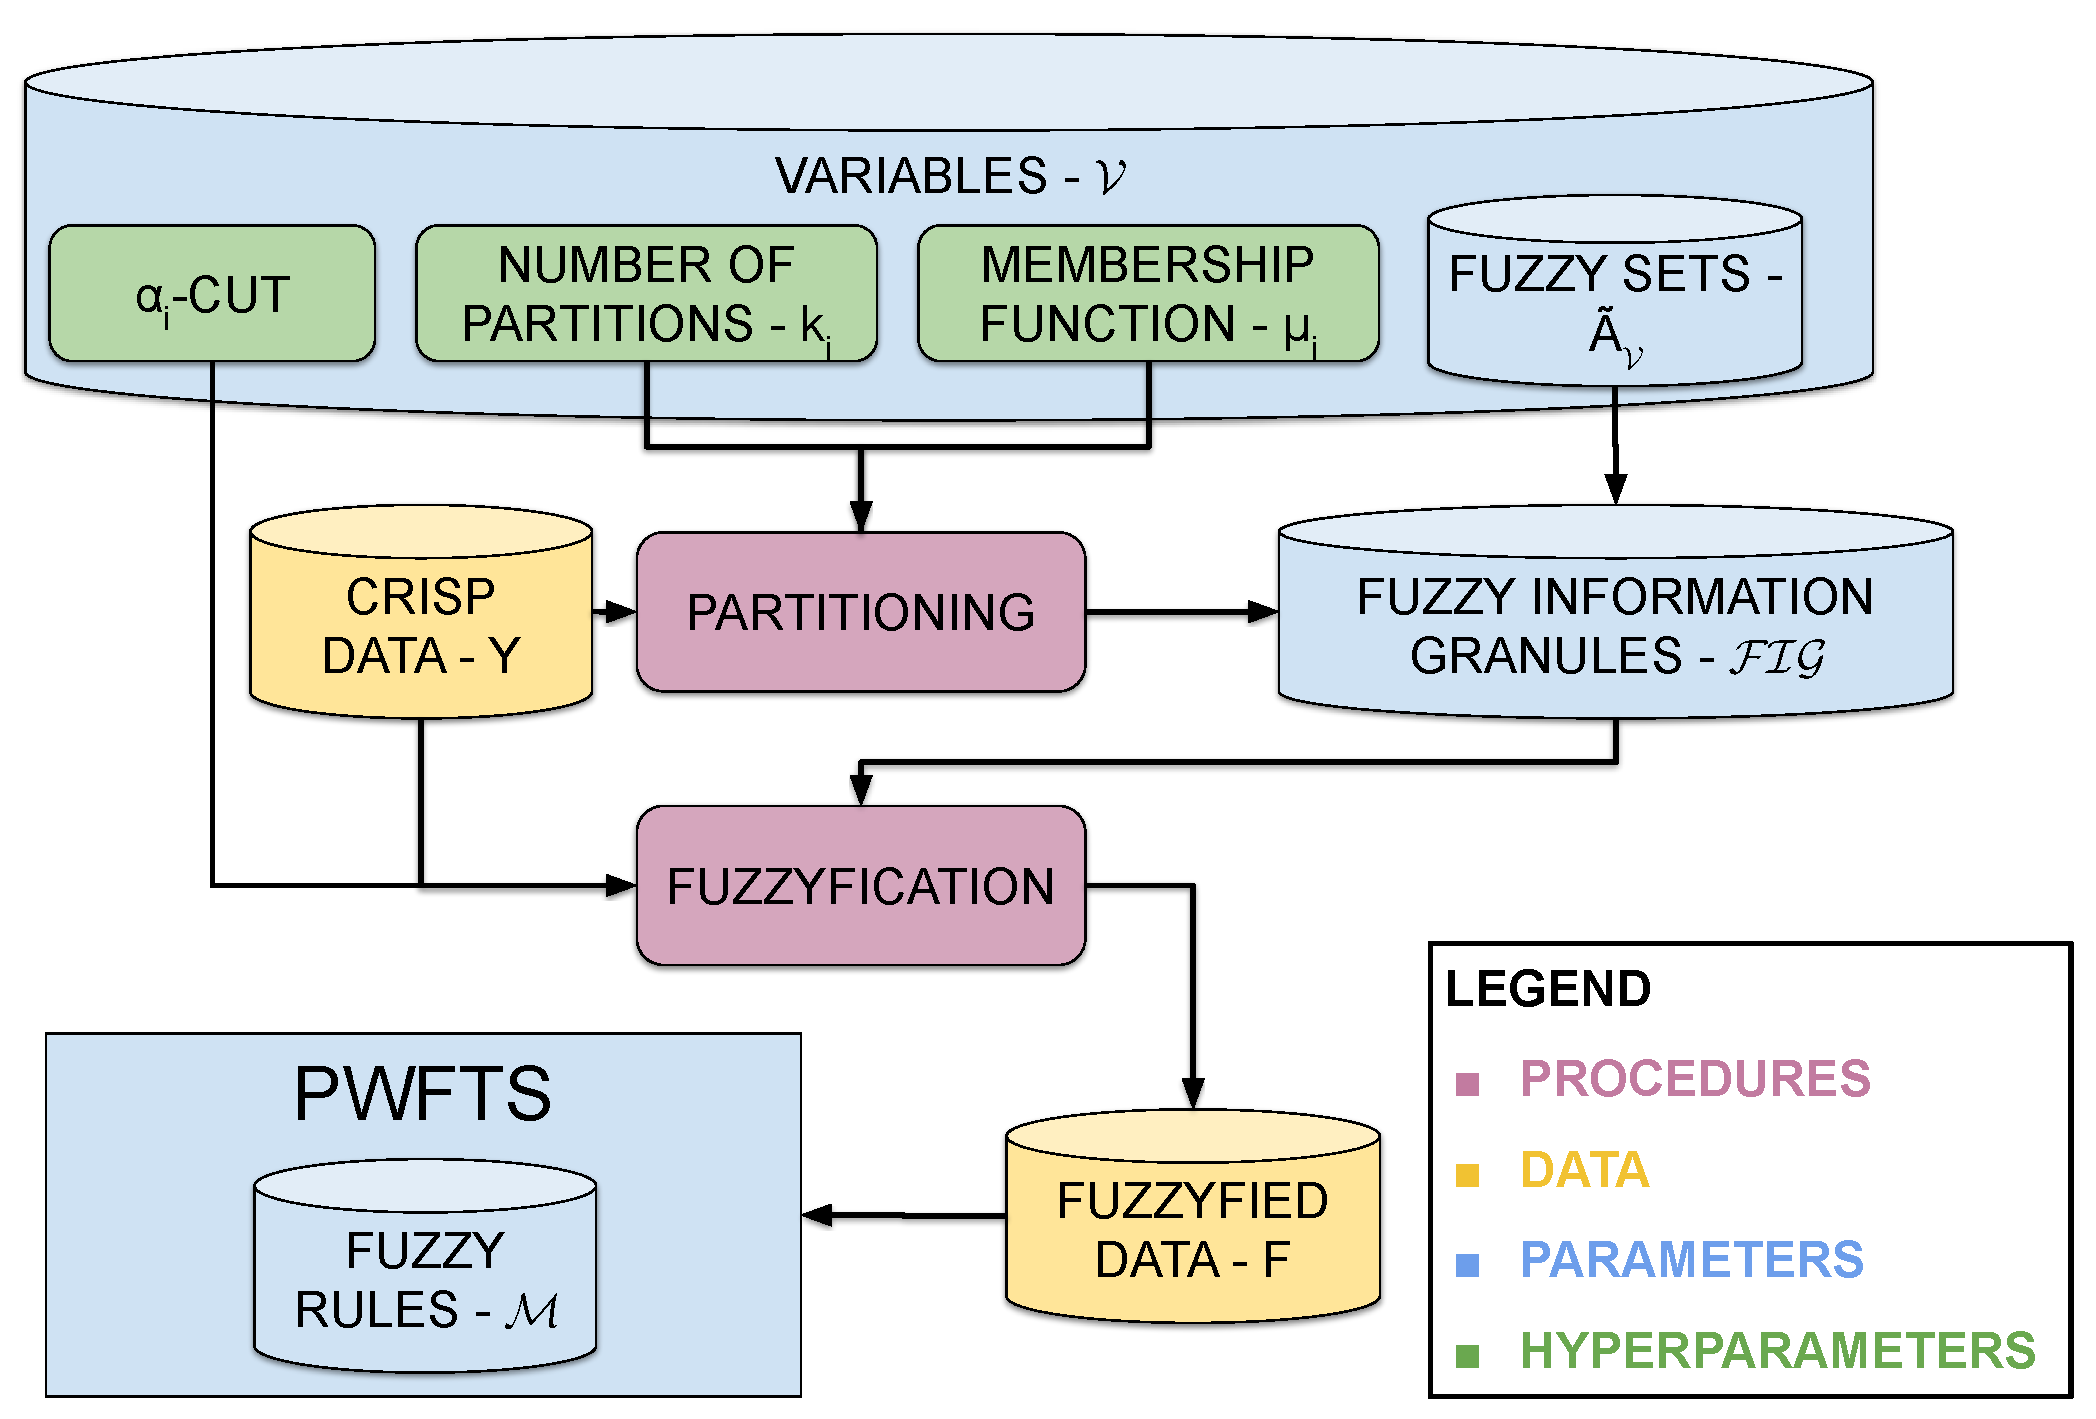
\includegraphics[width=\textwidth]{figures/figfts_training_procedure.pdf}
\caption{$\mathcal{FIG}$-FTS training procedure} 
\label{fig:figfts_training_procedure}
\end{figure}

\begin{enumerate}
\item[Stage 1] \textit{Partitioning}:
\begin{enumerate}
\item \textit{Defining $U_{\vari}$}: The Universe of Discourse $U_{\vari}$ defines the sample space, i.e., the known bounds of the variable $\vari$, such that $U_{\vari} = [\min(Y^{\vari})-D_1, \max(Y^{\vari})+D_2]$, where $D_1 = \min(Y^{\vari})\times 0.2$ and $D_2 = \max(Y^{\vari})\times 0.2$ are used to extrapolate the known bounds as a security margin, $\forall \vari \in \var$.

\item \textit{$U_{\vari}$ Partitioning}: Split $U_{\vari}$ in $k_i$ intervals $U_j$ with midpoints $c_j$, for $j=0..k_i$, where all the intervals have the same length;

\item \textit{Define the linguistic variable $\mlvar$}: For each interval $U_j \in U_{\vari}$  create an overlapping fuzzy set $\mfset$, with the membership function $\mu_{\mfset}(y_{\vari}(t))$, where $y_{\vari}(t)$ is the value of the $\vari$ variable on instance $y(t) \in Y$. The midpoint of the fuzzy set $\mfset$ will be $c_j$, the lower bound $l_j = c_{j-1}$ and the upper bound $u_j = c_{j+1}$ $\forall$ $j >0$ and $j < k_i$, and $l_0 = \min U_{\vari}$, $l_k = \max U_{\vari}$. Each fuzzy set $\mfset$ is a linguistic term of the linguistic variable $\mlvar$;

\end{enumerate}

\item[Stage 2] \textit{Fuzzyfication}: 

Transform the original numeric time series $Y$ into a fuzzy time series $F$, where each data point $f(t) \in F$ is a $\fig_i \in \FIG$. For each $y(t) \in Y$ the following steps must be executed:

\begin{enumerate}
    \item \textit{Individual variable fuzzyfication}: For each variable $\vari \in \var$, find the linguistic terms $\mfset \in \mlvar$, where the fuzzy membership is greater than the predefined $\alpha$-cut, i.e., $f_{\vari}(t) = \{\mfset\; |\; \mu_{\mfset}(y_{\vari}(t)) \geq \alpha_i\;\forall \mfset \in \mlvar\}$;
    
    \item \textit{Search in $\FIG$}: For each combination of fuzzy sets $\mfset$ in $f_{\vari}(t)$ verify if there is a $\figi \in \fig$ where $\figi \supset \{ \mfset \}, \forall \mfset \in f_{\vari}(t)$. If it exists, then the fuzzyfied value of $y(t)$ is $\figi$. This search is performed with KD-trees, comparing the midpoints of the fuzzyfied data and the midpoints of the fuzzy sets in the $\FIG$.
    
    \item \textit{Create new $\figi$ in $\FIG$}: If no $\figi$ was found in the previous step, new ones are added to $\FIG$. For each combination of fuzzy sets $\mfset$ in $f_{\vari}(t)$ create a fuzzy information granule $\figi$ such that $\figi = \{ \mfset \}, \forall \mfset \in f_{\vari}(t)$ and $\mu_{\fig_i} = \bigcap \mu_{\mfset}$. The created $\figi$ is then the fuzzyfied value of $y(t)$.
\end{enumerate}


\item[Stage 3] \textit{Rule Induction}: 
\begin{enumerate}
\item The fuzzyfied data $F$ where $f(t) = [(\fig_0,\mu_{\fig_0}),\ldots,(\figi,\mu_{\figi})]$ is passed to the Rule Induction stage of PWFTS method, which create the PWFTPG model $\model$. Each high-order PWFTG rule now will have the format $\pi_j \fig_{i0},...,\fig_{i\Omega} \rightarrow w_{j0} \cdot \fig_{i0}, \ldots w_{ji} \cdot \fig_{ji}$, where the LHS is $f(t - L(\Omega)) = \fig_{i0}$, $f(t - L(\Omega-1)) = \fig_{i1}$, ..., $f(t - L(0)) = \fig_{i\Omega}$ and the RHS is $f(t+1) \in \{\fig_k, \fig_j,...\}$ and the weights $\pi_j, w_{jk}$ are the fuzzy empirical probabilities.
\end{enumerate}
\end{enumerate}


%%%%%%%%%%%%%%%%%%%%%%%%%%%%%%%%%%%%%%%%%%%%%%%%%%%%%%%%%
%%%%%%%%%%%%%%%%%%%%%%%%%%%%%%%%%%%%%%%%%%%%%%%%%%%%%%%%%
\subsection{Forecasting Procedure} 
\label{sec:fig_forecasting_procedure}

\begin{figure}
\centering
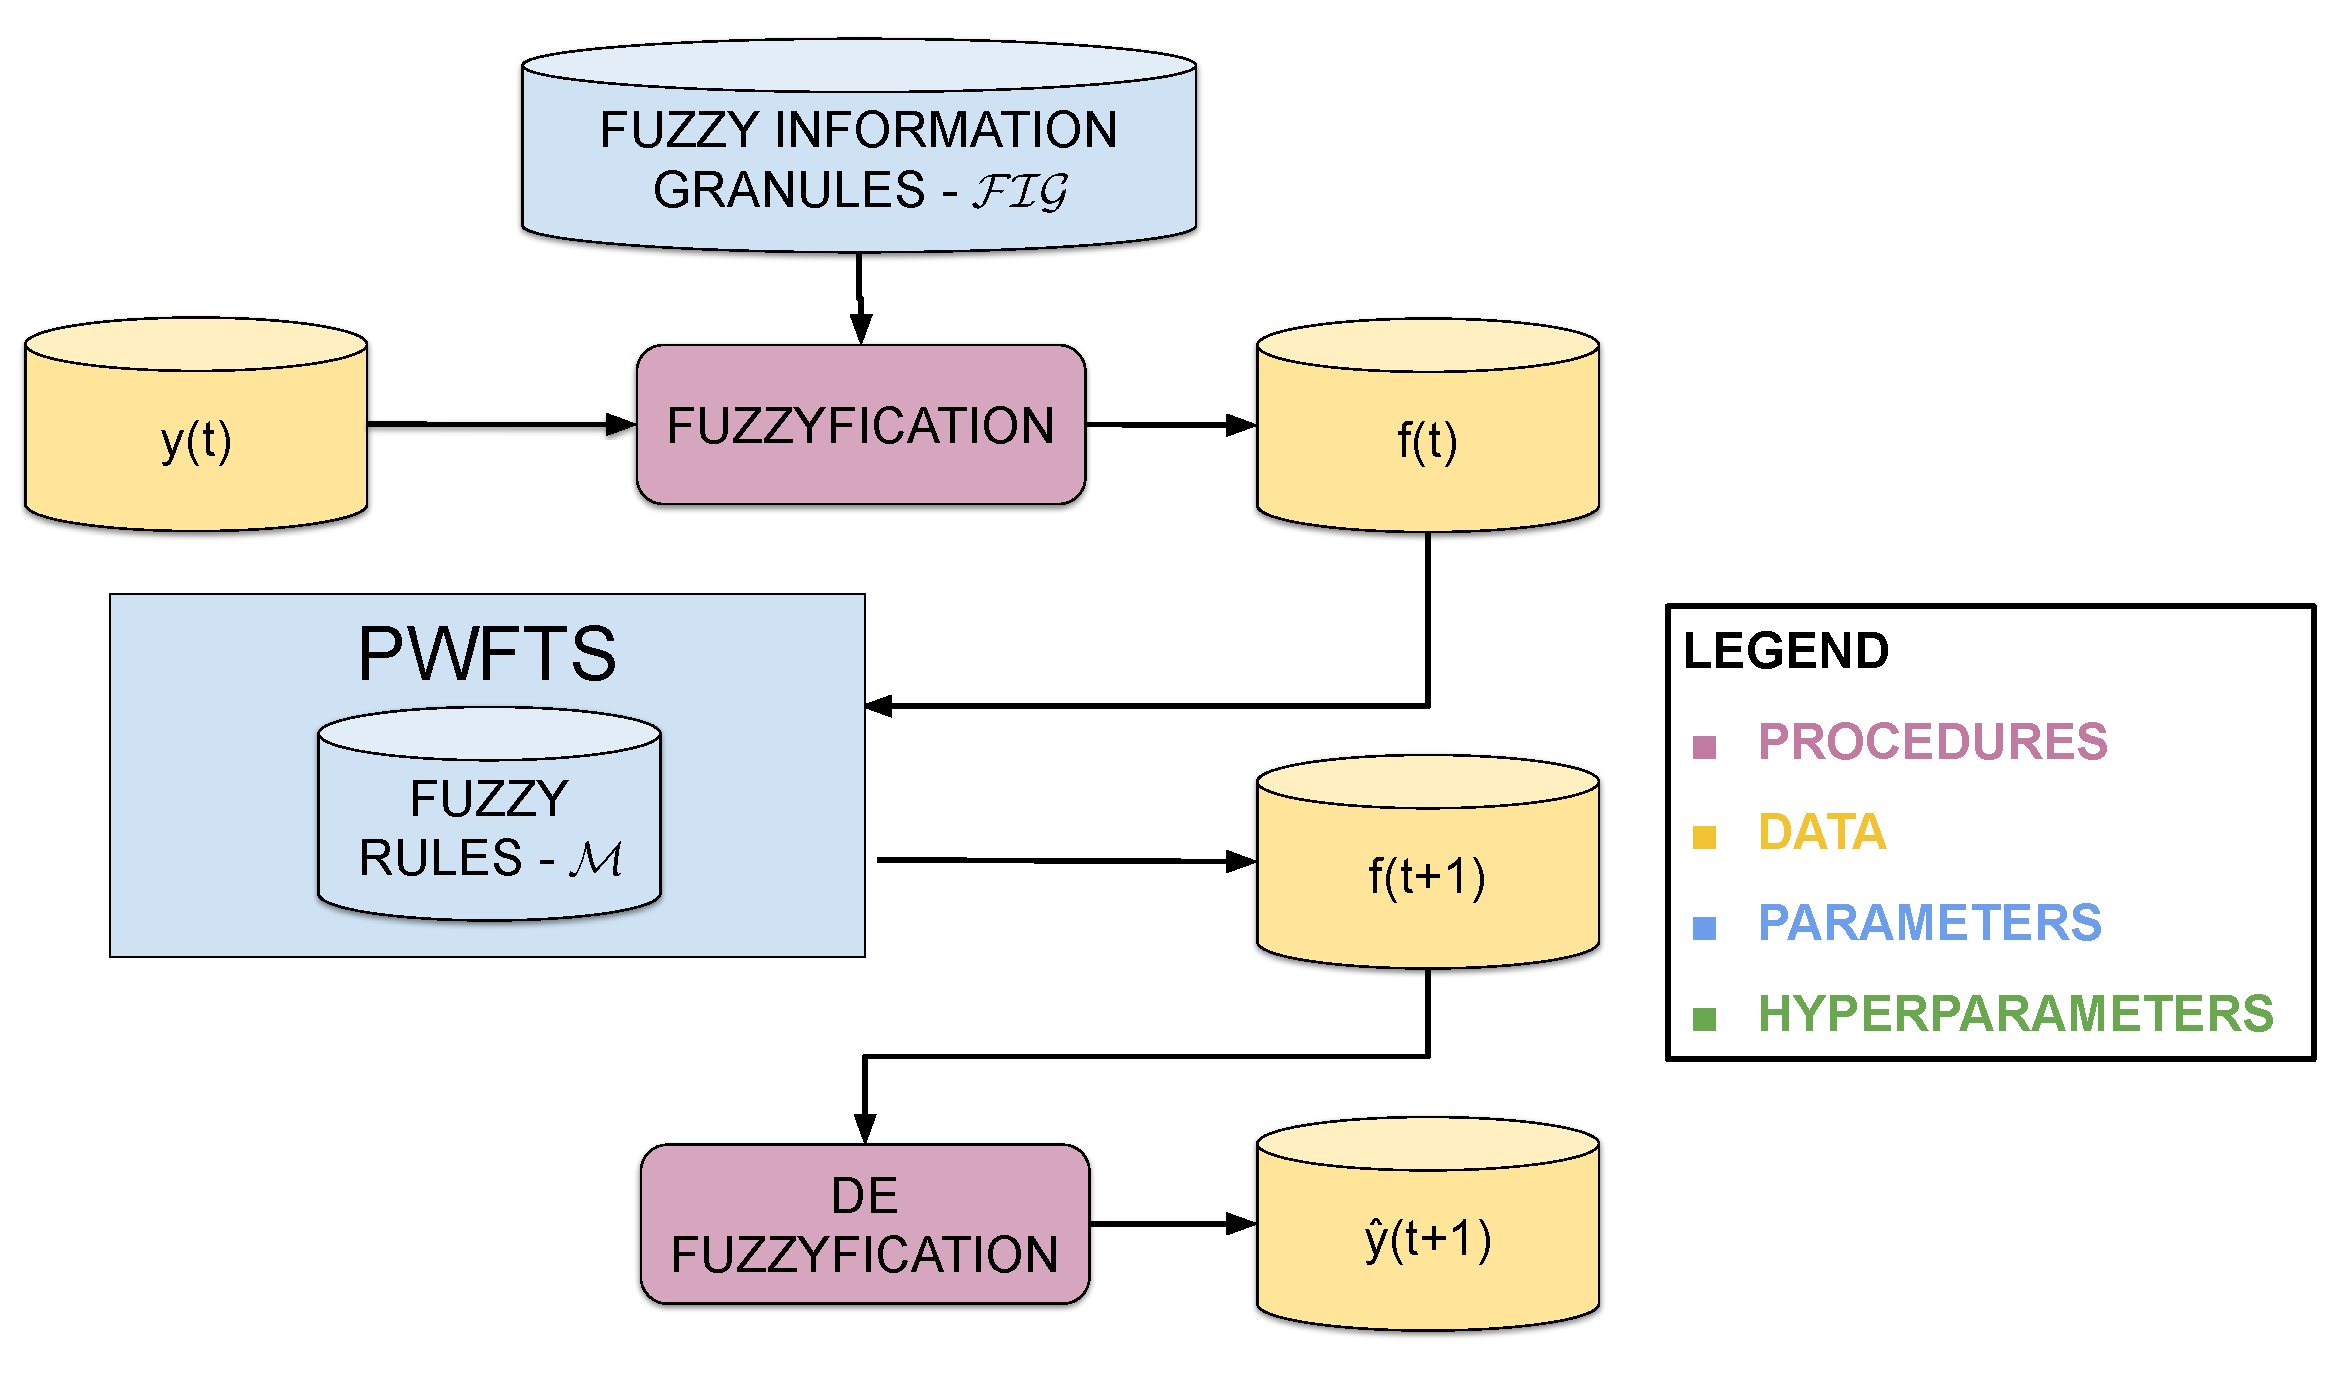
\includegraphics[width=\textwidth]{figures/figfts_forecasting_procedure.pdf}
\caption{$\mathcal{FIG}$-FTS forecasting procedure} 
\label{fig:figfts_forecasting_procedure}
\end{figure}

\begin{enumerate}
\item [Step 1] \textit{Fuzzyfication}: Find the $\kappa$ closest   $\fig_{i\Omega},...,\fig_{i0} \in \FIG$ to the input sample $y(t-\Omega),...,y(t)$. 

\item [Step 2] \textit{Rule matching}: The fuzzyfied input sample is transfered to PWFTS that search for the applicable rules. For each PWFTPG rule $j$ found, its fuzzy membership is given by:
\begin{equation}
    \mu_j = \bigcap_{t\in L\; i \in \FIG} \mu_{\fig_{it}}
\end{equation}

\item [Step 3] \textit{Defuzzyfication}: 
\begin{enumerate}
    \item \textit{Target variable selection}: For non multivariate forecasts a target variable $*\var$ must be chosen between the variables $\var$.
    \item \textit{PWFTPG adaption}: After the target variable $*\var$ be selected, the RHS of all PWFTPG's are modified, replacing the $figi$ by the fuzzy sets $\tfset \in *\mlvar$, keeping the weights untouched;
    \item \textit{Deffuzyfication}: The PWFTS deffuzyfication methods (point, interval and probabilistic) can be invoked without modifications;
\end{enumerate}

\item [Step 4] \textit{Multivariate forecasting}:
\begin{enumerate}
    \item If a target variable was not specified, compute a point forecast $\hat{y}^{\vari}(t+1)$ invoking the PWFTS point forecasting by taking each variable $\vari \in \var$ as a target variable;
    \item Merge the individual variable forecastings to create the multivariate forecast $\hat{y}(t+1) = \bigcup_{\vari \in \var} \hat{y}^{\vari}(t+1)$ 
\end{enumerate}
 
\item [Step 5] \textit{Forecasting horizon}: Given the number $m$ of steps ahead to forecast  (the forecast horizon), repeat the Steps 1 to 4 $m$ times, appending the output $\hat{y}$ of the previous Step 4 at the end of the $y(t)$ input for the next Step 1.
\end{enumerate}

\subsection{Method discussion}
\label{sec:fig_discussion}

The main insight of the $\mathcal{FIG}$-FTS is that the linguistic variables $\mlvar$ work as feature extraction layers and each fuzzy information granule $\fig$ is a small cluster prototype of these features, simplifying the representation of temporal patterns and aiding pattern identification and rule induction. Each $\fig$ also helps the multivariate defuzzyfication process, working as a final output layer for the model.

The learning procedure of $\FIG$-FTS is controlled by its hyperparameters that directly affect its accuracy and parsimony. The number of partitions of each variable $k_i$ affects the number of rules directly, given the maximum number of rules (in the worst case) is a Cartesian product of the fuzzy sets $\mfset \in \mlvar$, for each $\vari \in \var$. The $\alpha_i$-cut, on the other hand, controls the fuzzyfication sensibility by eliminating, in  the rule induction stage, values with lower membership grades. It reduces the number of rules by preventing the capture of spurious patterns, generated by insignificant memberships or noise. The $\alpha_i$-cut also enhances the forecasting process by eliminating lower related rules on rule search.

The parameter $\kappa$ has influence on the forecasting accuracy. There is also a balance between the use of too few or too many rules on forecasting procedure, such that too few rules may not have enough patterns to describe the correct time series behavior and too many may bring patterns that are not closely related with the current behavior.

In the next section the empirical results of the proposed method are presented, showing its effectiveness for complex artificial and natural dynamic processes.

%%%%%%%%%%%%%%%%%%%%%%%%%%%%%%%%%%%%%%%%%%%%%%%%%%%%%%%%%
%%%%%%%%%%%%%%%%%%%%%%%%%%%%%%%%%%%%%%%%%%%%%%%%%%%%%%%%%
\section{Computational Experiments}
\label{sec:multivariate_experiments}

This section presents an exploratory study of multivariate FTS methods and $\mathcal{FIG}$-FTS. The computational experiments employed two multivariate time series, the SONDA dataset with 2,000,000 instances and the Malaysia dataset, with 17,000 instances. Both datasets are detailed in Appendix \ref{apd:multivariate_datasets}, where its main characteristics are presented.

The multivariate models were testes for point, interval and probabilistic forecasting (in the case of $\mathcal{FIG}$-FTS) using the presented FTS methods as competitor models. For each dataset, with exception to timestamp variables, each variable $\vari \in \var$ was used as target variable $*\var$ once, allowing the comparation with the monovariate FTS methods. 

In order to optimize the forecasting accuracy an specific configuration of variables was researched for each $*\var \in \var$, and it is shared among MVFTS, WMVFTS and  $\FIG$-FTS. The specific values of $k_i$, $\mu_i$ and $\alpha_i$ for each variable $\vari \in \var$ were obtained using DEHO method on the isolated variables.

In subsections \ref{sec:variables_sonda} and \ref{sec:variables_malaysia} the details about the variables of the multivariate methods are presented. In subsection \ref{sec:multivariate_results} the results of the experiments are presented for point, interval and probabilistic forecasting, and samples of methods performances are provided.

In order to contribute with the replication of all the results in the research, all data and source codes employed in this chapter are available at the URL:
\texttt{\url{http://bit.ly/scalable_probabilistic_fts_chap6}}

%%%%%%%%%%%%%%%%%%%%%%%%%%%%%%%%%%%%%%%%%%%%%%%%%%%%%%%%%
%%%%%%%%%%%%%%%%%%%%%%%%%%%%%%%%%%%%%%%%%%%%%%%%%%%%%%%%%
\subsection{SONDA models settings}
\label{sec:variables_sonda}

The SONDA dataset is composed by 3 variables \texttt{DateTime} (timestap of each instance), \texttt{glo\_avg} (solar radiation) and \texttt{ws\_10m} (wind speed). The details of this dataset and its variables are presented in Appendix \ref{apd:multivariate_datasets}. 

The Solar Radiation variable, is independent to Wind Speed variable and then this last can be discard. The Solar Radiation has two main seasonal components: yearly and hourly. These two seasonalities can be extracted from the DateTime variable.  A model to forecast the Solar Radiation variable based on SONDA  multivariate dataset contains the set up presented in Table \ref{tab:variables_sonda_solar} and illustrated in Figure \ref{fig:variables_sonda_solar}.

\begin{table}[htb]
    \centering
    \begin{tabular}{|c|c|c|c|c|} \hline
        $\mathbf{\vari}$ & \textbf{Data Source} & $\mathbf{k_i}$ & $\mathbf{\mu_i}$ & $\mathbf{\alpha_i}$  \\ \hline
        Hour & DateTime & 24 & Triangular & .3 \\ \hline 
        Month & DateTime & 12 & Triangular & .3 \\ \hline 
        Solar & glo\_avg & 5 & Gaussian & .25 \\ \hline 
    \end{tabular}
    \caption{Variables and partitioning for SONDA Solar Radiation}
    \label{tab:variables_sonda_solar}
\end{table}

The Wind Speed variable is independent to Solar Radiation variable and then this last can be discard. The Wind Speed has a yearly seasonal components that can be extracted from the DateTime variable.  A model to forecast the Wind Speed variable based on SONDA  multivariate dataset contains the set up presented in Table \ref{tab:variables_sonda_wind} and illustrated in Figure \ref{fig:variables_sonda_wind}.

\begin{figure}[htb]
    \centering
    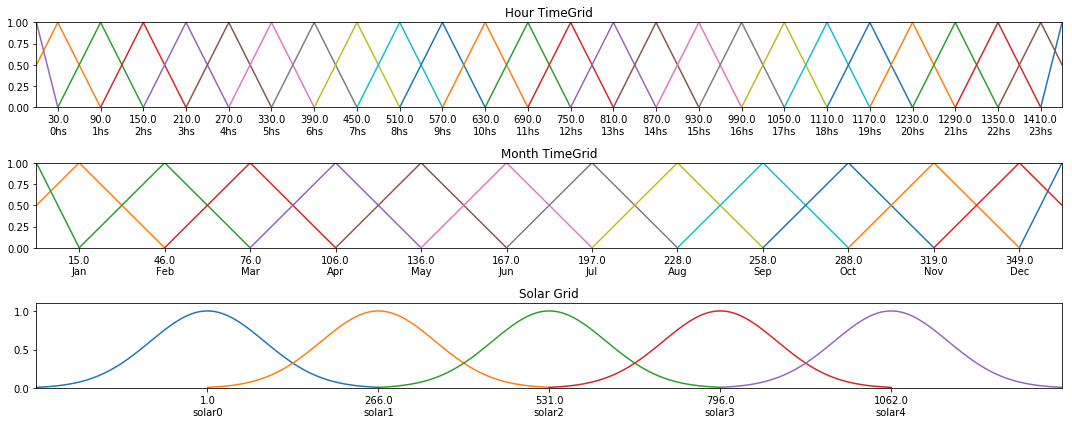
\includegraphics[width=\textwidth]{figures/variables_sonda_solar.png}
    \caption{Variables and partitioning for SONDA Solar Radiation}
    \label{fig:variables_sonda_solar}
\end{figure}

\begin{table}[htb]
    \centering
    \begin{tabular}{|c|c|c|c|c|} \hline
        $\mathbf{\vari}$ & \textbf{Data Source} & $\mathbf{k_i}$ & $\mathbf{\mu_i}$ & $\mathbf{\alpha_i}$  \\ \hline
        Month & DateTime & 12 & Triangular & .3 \\ \hline 
        Wind & ws\_10m & 15 & Gaussian & .25 \\ \hline 
    \end{tabular}
    \caption{Variables and partitioning for SONDA Solar Radiation}
    \label{tab:variables_sonda_wind}
\end{table}

\begin{figure}[htb]
    \centering
    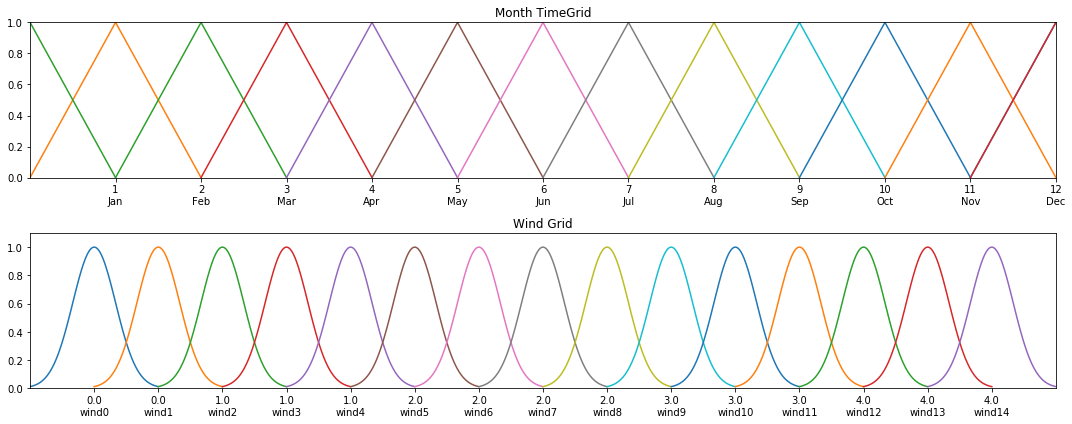
\includegraphics[width=\textwidth]{figures/variables_sonda_wind.png}
    \caption{Variables and partitioning for SONDA Wind Speed}
    \label{fig:variables_sonda_wind}
\end{figure}

%%%%%%%%%%%%%%%%%%%%%%%%%%%%%%%%%%%%%%%%%%%%%%%%%%%%%%%%%
%%%%%%%%%%%%%%%%%%%%%%%%%%%%%%%%%%%%%%%%%%%%%%%%%%%%%%%%%
\subsection{Malaysia models settings}
\label{sec:variables_malaysia}

The Malaysia dataset is composed by 3 variables \texttt{DateTime} (timestap of each instance), \texttt{temperature} and \texttt{load} (electric load). The details of this dataset are presented in Appendix \ref{apd:multivariate_datasets}.

The Load variable is a hourly seasonal variable (e. g. dependent of DateTime variable) and also known to be dependent of the temperature variable. A model to forecast the Load variable based on Malaysia multivariate dataset contains the set up presented in Table \ref{tab:variables_malaysia_load} and illustrated in Figure \ref{fig:variables_malaysia_load}. 

\begin{table}[htb]
    \centering
    \begin{tabular}{|c|c|c|c|c|} \hline
        $\mathbf{\vari}$ & \textbf{Data Source} & $\mathbf{k_i}$ & $\mathbf{\mu_i}$ & $\mathbf{\alpha_i}$  \\ \hline
        Hour & DateTime & 24 & Triangular & .3 \\ \hline 
        Temperature & temperature & 10 & Gaussian & .3 \\ \hline 
        Load & load & 10 & Gaussian & .25 \\ \hline 
    \end{tabular}
    \caption{Variables and partitioning for SONDA Solar Radiation}
    \label{tab:variables_malaysia_load}
\end{table}

\begin{figure}[htb]
    \centering
    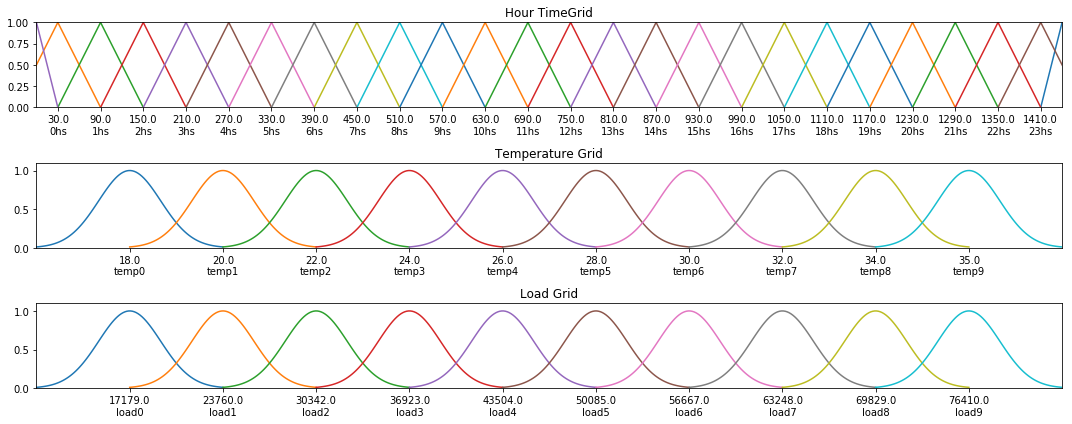
\includegraphics[width=\textwidth]{figures/variables_malaysia.png}
    \caption{Variables and partitioning for Malaysia Eletric Load}
    \label{fig:variables_malaysia_load}
\end{figure}

The Temperature variable, in other hand, is independent in relation of Load variable and then it can be discarded. The temperature has two main seasonal components: yearly and hourly. These two seasonalities can be extracted from the DateTime variable.  A model to forecast the Temperature variable based on Malaysia multivariate dataset contains the set up presented in Table \ref{tab:variables_malaysia_temperature} and illustrated in Figure \ref{fig:variables_malaysia_temperature}.

\begin{table}[htb]
    \centering
    \begin{tabular}{|c|c|c|c|c|} \hline
        $\mathbf{\vari}$ & \textbf{Data Source} & $\mathbf{k_i}$ & $\mathbf{\mu_i}$ & $\mathbf{\alpha_i}$  \\ \hline
        Hour & DateTime & 24 & Triangular & .3 \\ \hline 
        Month & DateTime & 12 & Triangular & .3 \\ \hline 
        Temperature & temperature & 10 & Gaussian & .3 \\ \hline 
    \end{tabular}
    \caption{Variables and partitioning for Malaysia Temperature}
    \label{tab:variables_malaysia_temperature}
\end{table}

\begin{figure}[htb]
    \centering
    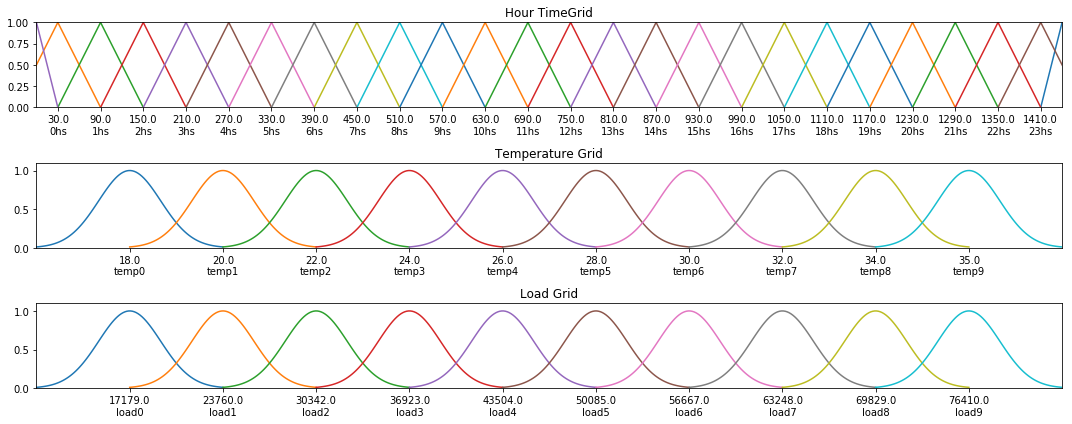
\includegraphics[width=\textwidth]{figures/variables_malaysia.png}
    \caption{Variables and partitioning for Malaysia Temperature}
    \label{fig:variables_malaysia_temperature}
\end{figure}

%%%%%%%%%%%%%%%%%%%%%%%%%%%%%%%%%%%%%%%%%%%%%%%%%%%%%%%%%
%%%%%%%%%%%%%%%%%%%%%%%%%%%%%%%%%%%%%%%%%%%%%%%%%%%%%%%%%
\subsection{Results}
\label{sec:multivariate_results}

The RMSE accuracy for one step ahead point forecasting is presented in Figure \ref{fig:multivariate_point_results}, by method and dataset. Samples of the multivariate methods point forecasting performance are also illustrated in Figure \ref{fig:multivariate_sample_onestep} for one step ahead forecasting and in Figure \ref{fig:multivariate_sample_manystep} for many steps ahead forecasting.

\begin{figure}[htb]
    \centering
    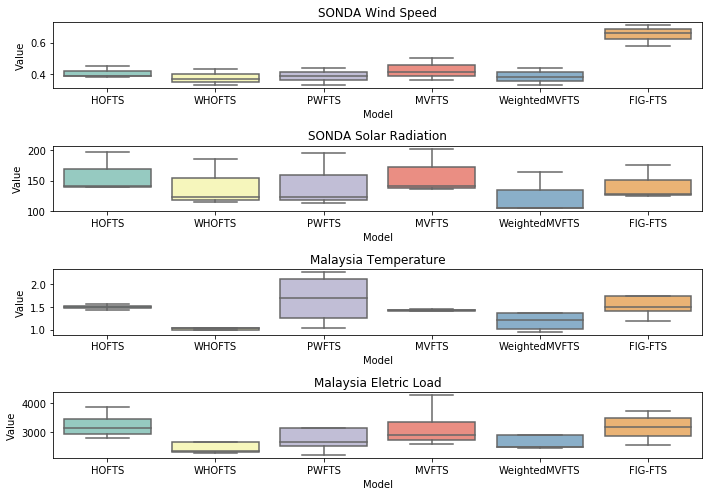
\includegraphics[width=\textwidth]{figures/multivariate_point_results.png}
    \caption{RMSE point forecasting accuracy for one step ahead}
    \label{fig:multivariate_point_results}
\end{figure}

\begin{figure}[htb]
    \centering
    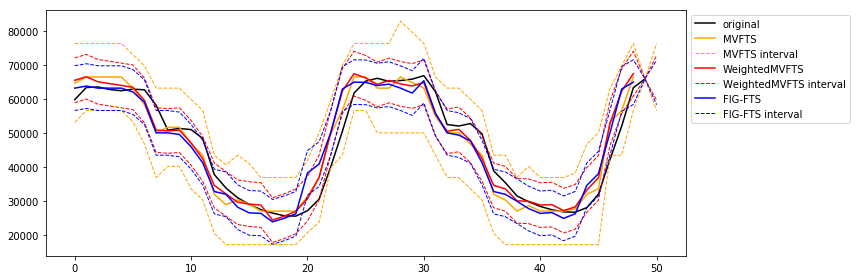
\includegraphics[width=\textwidth]{figures/multivariate_sample_onestep.png}
    \caption{Sample of point and interval forecasts for one step ahead by multivariate method}
    \label{fig:multivariate_sample_onestep}
\end{figure}

\begin{figure}[htb]
    \centering
    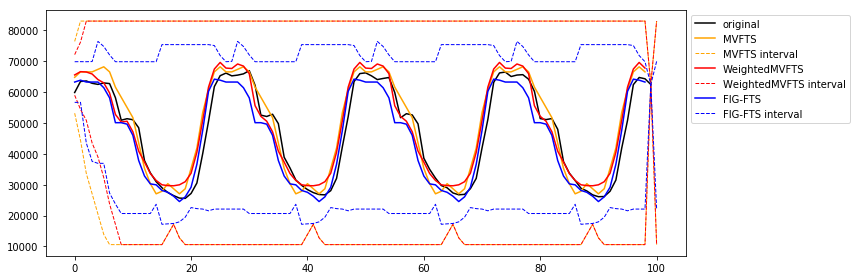
\includegraphics[width=\textwidth]{figures/multivariate_sample_manystep.png}
    \caption{Sample of point and interval forecasts for many steps ahead by multivariate method}
    \label{fig:multivariate_sample_manystep}
\end{figure}

The interval forecasting accuracy using the Winkler Score metric, for one step ahead is presented in Figure \ref{fig:multivariate_interval_results}, by method and dataset. Samples of the multivariate methods interval forecasting performance are also illustrated in Figure \ref{fig:multivariate_sample_onestep} for one step ahead forecasting and in Figure \ref{fig:multivariate_sample_manystep} for many steps ahead forecasting.

\begin{figure}[htb]
    \centering
    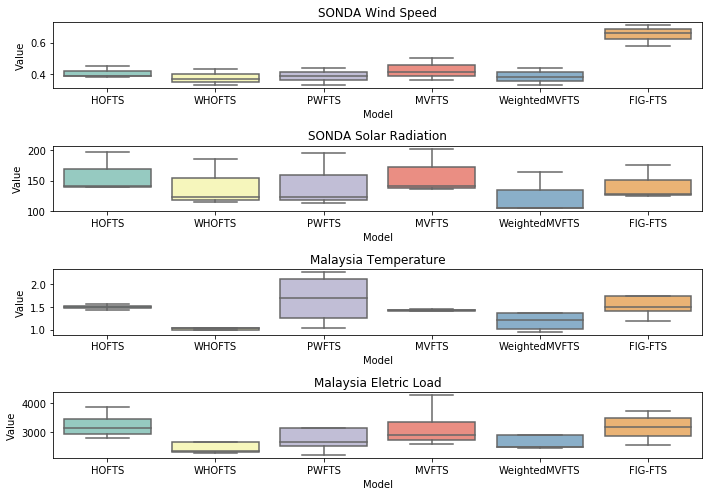
\includegraphics[width=\textwidth]{figures/multivariate_point_results.png}
    \caption{Winkler interval forecasting accuracy for one step ahead}
    \label{fig:multivariate_interval_results}
\end{figure}

The probabilistic forecasting accuracy using the CRPS metric, for one step ahead, is presented in Figure \ref{fig:multivariate_probabilistic_results}, by method and dataset. Samples of $\mathcal{FIG}$-FTS probabilistic forecasting performance are also illustrated in Figures \ref{fig:figfts_probabilistic_onestep} and \ref{fig:figfts_probabilistic_onestep_tiled} for one step ahead forecasting and in Figures \ref{fig:figfts_probabilistic_manystep} and \ref{fig:figfts_probabilistic_manystep_tiled} for many steps ahead forecasting.

\begin{figure}[htb]
    \centering
    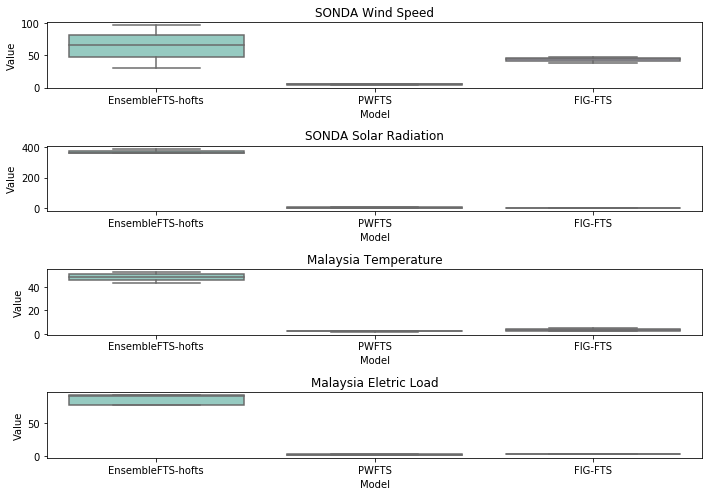
\includegraphics[width=\textwidth]{figures/multivariate_probabilistic_results.png}
    \caption{CRPS probabilistic forecasting accuracy for one step ahead}
    \label{fig:multivariate_probabilistic_results}
\end{figure}

\begin{figure}[htb]
    \centering
    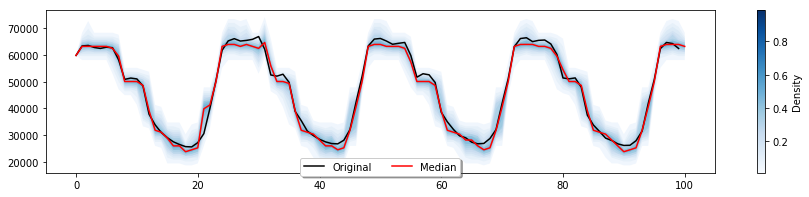
\includegraphics[width=\textwidth]{figures/figfts_probabilistic_onestep.png}
    \caption{Sample of $\mathcal{FIG}$-FTS probabilistic forecasting for one step ahead}
    \label{fig:figfts_probabilistic_onestep}
\end{figure}

\begin{figure}[htb]
    \centering
    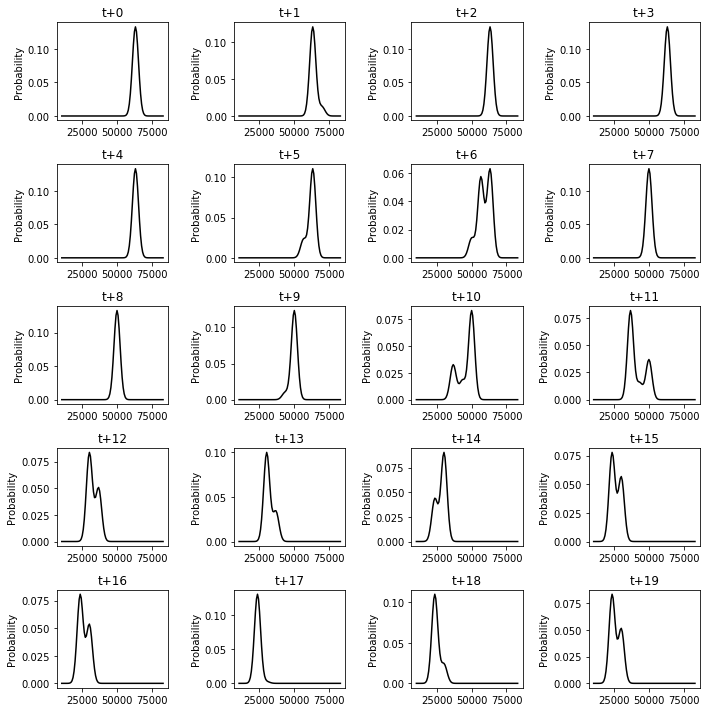
\includegraphics[width=\textwidth]{figures/figfts_probabilistic_onestep_tiled.png}
    \caption{Shape of $\FIG$-FTS probabilistic distributions for one step ahead}
    \label{fig:figfts_probabilistic_onestep_tiled}
\end{figure}


\begin{figure}[htb]
    \centering
    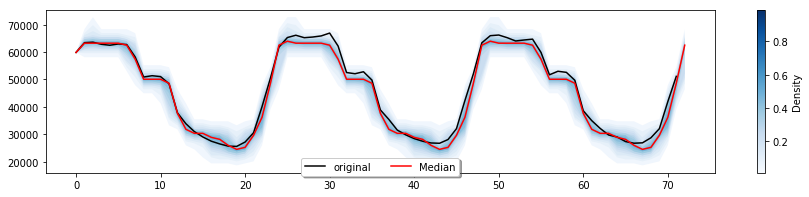
\includegraphics[width=\textwidth]{figures/figfts_probabilistic_manystep.png}
    \caption{Sample of $\mathcal{FIG}$-FTS probabilistic forecasting for many steps ahead}
    \label{fig:figfts_probabilistic_manystep}
\end{figure}

\begin{figure}[htb]
    \centering
    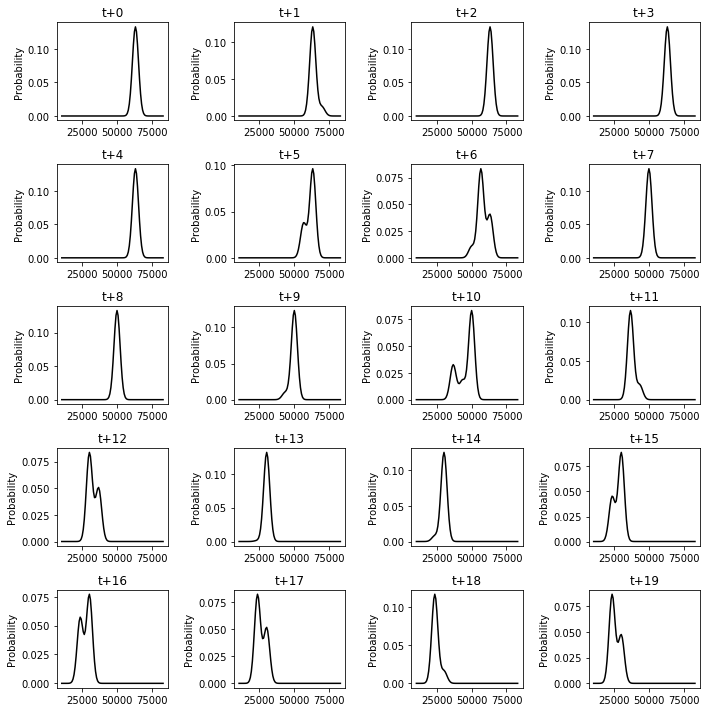
\includegraphics[width=\textwidth]{figures/figfts_probabilistic_manystep_tiled.png}
    \caption{Shape of $\mathcal{FIG}$-FTS probabilistic distributions for many steps ahead}
    \label{fig:figfts_probabilistic_manystep_tiled}
\end{figure}

%%%%%%%%%%%%%%%%%%%%%%%%%%%%%%%%%%%%%%%%%%%%%%%%%%%%%%%%%
%%%%%%%%%%%%%%%%%%%%%%%%%%%%%%%%%%%%%%%%%%%%%%%%%%%%%%%%%
\section{Conclusion}
\label{sec:multivariate_conclusion}

Accurate forecasting of complex dynamics systems, as several natural and social processes, is a challenging task specially when the underlying system is composed by many interacting variables. For FTS methods, dealing with multivariate and spatio-temporal time series was always a challenging task, specially because of the complexity growth of the rules as the number of variables increases.

This section presented a short overview of multivariate FTS methods, focusing on the rule based conventional Multivariate Fuzzy Time Series (MVFTS) and its weighted version WMVFTS. 

In order to extend the PWFTS method to multivariate time series, the method Fuzzy Information Granule FTS ($FIG$-FTS) was proposed. $FIG$-FTS is a wrapper method that pre-process the multivariate input translating it onto a monovariate and allowing its use by monovariate methods. $\FIG$-FTS makes use of Fuzzy Information Granules (FIG), which in this work is a multivariate fuzzy set incrementally created during the fuzzyfication stage.

With $\FIG$-FTS, the PWFTS extends its foreasting capabilities to multivariate data, being the first multivariate FTS method to forecast points, intervals and probability distributions. 

\subsection{Method limitations}

$\FIG$-FTS produces non-parsimonious methods that can be computationally expensive. In order to optimize the models, both in terms of accuracy and parsimony, it is advisable to fine tunning the hyperparameters of each variable, as well as to optimize the choose of the best variables of the model.